\documentclass[11pt,a4paper, twocolumn,
swedish, english %% Make sure to put the main language last!
]{article}
\pdfoutput=1

%% Andréas's custom package 
%% (Will work for most purposes, but is mainly focused on physics.)
\usepackage{custom_as}

%% Figures can now be put in a folder: 
\graphicspath{ {figures/} %{some_folder_name/}
}

%% If you want to change the margins for just the captions
\usepackage[size=small]{caption}

%% To add todo-notes in the pdf
\usepackage[%disable  %%this will hide all notes
]{todonotes} 

%% Change the margin in the documents
\usepackage[
%            top    = 3cm,              %% top margin
%            bottom = 3cm,              %% bottom margin
             left   = 1.2cm, right  = 1.2cm %% left and right margins
]{geometry}


%% If you want to change the formatting of the section headers
%\renewcommand{\thesection}{...}

\newcommand{\rr}{\mathrm{r}}

%%%%%%%%%%%%%%%%%%%%%%%%%%%%%%%%%%%%%%%%%%%%%%%%%%%%%%%%%%%%%%%%%%%%%%
\begin{document}%% v v v v v v v v v v v v v v v v v v v v v v v v v v
%%%%%%%%%%%%%%%%%%%%%%%%%%%%%%%%%%%%%%%%%%%%%%%%%%%%%%%%%%%%%%%%%%%%%%


%%%%%%%%%%%%%%%%%%%% vvv Internal title page vvv %%%%%%%%%%%%%%%%%%%%%
\title{SALSA project report}
\author{Andréas Sundström}
\date{\today}


\twocolumn[
\begin{@twocolumnfalse}
\maketitle
\begin{abstract}

\end{abstract}
\end{@twocolumnfalse}
]


%%%%%%%%%%%%%%%%%%%% ^^^ Internal title page ^^^ %%%%%%%%%%%%%%%%%%%%%
%% If you want a list of all todos
%\todolist

\section{Introduction}
The interstellar medium (ISM) contains clouds, among others, atomic
hydrogen HI, which trough quantum mechanical hyperfine structure
electronic transitions emits electromagnetic radiation with a
frequency of about 1420\,MHz corresponding to a wavelength of
21\,cm. This frequency then gets Doppler shifted depending on the
relative radial velocity between us and the cloud. Therefore by
observing the frequency spectrum of the incoming radiation in the
21\,cm band, it is possible to determine the presence and relative
radial velocity of clouds in the line of sight.
Once a rotation curve has been established, it can be used to
determine the positions of these clouds.

In this report we use the SALSA 2.4\,m radio telescopes a Onsala Space
Observatory to scan a portion of the Galaxy, that is visible from Onsala,
in the 21\,cm band to find HI clouds. The Doppler shift is then used
to calculate the radial velocity of these clouds, as seen from
Earth. This is then used to determine the rotation curve and the
positions of the observed clouds.

\subsection{Galactic coordinates and measurements}
The Galactic longitude, $l$, of an object is the angle, as seen from
us, in the plane of the Galactic disc between the Galactic center (GC)
and the object in question. %, see \figref{fig:glon}.
The Galactic latitude is measured as the angle above the Galactic
plane. 

% \begin{figure}\centering
% \resizebox{0.4\linewidth}{!}{
% \input{figures/glon.pdf_t}}
% \caption{Illustration of Galactic coordinates. The Galactic longitude,
%   $l$, is measured as the angle between an object and the Galactic
%   center (GC). }
% \label{fig:glon}
% \end{figure}

\begin{figure}\centering
\resizebox{0.5\linewidth}{!}{
\input{figures/geom.pdf_t}}
\caption{The geometry of an HI measurement, as seen in the plane of
  the Galaxy. If there is a cloud on Galactic longitude $l$ on a circular
  orbit the observed radial velocity is $V_\rr=V\cos\alpha-V_0\sin l$. }
\label{fig:geom}
\end{figure}

Given the geometry of \figref{fig:geom}, the law of sines gives the
relation
\begin{equation}\label{eq:sine-law}
\frac{\sin l}{R_0}=\frac{\sin\beta}{R}
\end{equation}
Assuming circular orbits further gives $\beta=\alpha-\pi/2$.
This together with \eqref{eq:sine-law} means that observed radial
velocity has to be
\begin{equation}\label{eq:Vr}
V_\rr=V\cos\alpha-V_0\sin l
=\sin(l)\qty[\tfrac{R}{R_0}V-V_0].
\end{equation}
This is one equation with two unknowns\footnote{We already know 
  $R_0=\unit[8.5]{kpc}$ and $V_0=\unit[220]{km/s}$.}. To solve this 
we (highly dubiously) assume that the clouds we observe having the
highest radial velocity, $V_\rr$, are on a trajectory tangent to our
line of sight ($\alpha=0$). The justification for this that in each
direction looking into the Galaxy, we tend to observe two or three
clouds and therefor it is possible that one of those clods have
$\alpha=0$. If $\alpha=0$ then \eqref{eq:sine-law} yields
$R_0/R=\sin(l)$, or in other words
\begin{equation}
V=V_{\rr,\max}+V_0\sin l.
\end{equation}
We can now determine both $V$ and $R$ together, which makes it
possible to find  the rotation curve.

This is however only possible for when looking in towards the center
of the Galaxy, $0<l<\pi/2$ (or $3\pi/2<l<2\pi$), otherwise the
assumption of trajectorie tangential to the line of sight can not be
fulfilled. For $\pi/2<l<3\pi/2$, which also implies $R>R_0$, we cannot
observe the orbital velocity. Instead we just have to blindly hope
that the observed rotation curve extrapolates nicely to $R>R_0$.



\subsubsection{Position determination and ambiguity}
Assuming that we managed to get a rotation curve $V(R)$, and that it
can be extrapolated to all $R$, the position of the observed cloud can
be determined by first inverting \eqref{eq:Vr} to get $R$. Once we
have $R$, we need $d$ to fully determine the postion of the HI
cloud.

By the law of cosines, we have
\begin{equation}
R^2=R_0^2+d^2-2R_0d\cos l,
\end{equation}
which inverts to
\begin{equation}\label{eq:d}
d=R_0\cos l \pm\sqrt{R^2-R_0^2\sin^2l}.
\end{equation}
For $R>R_0$ it is clear that one of the above solution must be
negative, hence the cloud position is uniquely determined.
If, on the other hand, $R<R_0$ (which implies that $0<l<\pi/2$ or
$3\pi/2<l<2\pi$) there might be two positive solutions, which means
that $d$ could be ambiguous. This happens when 
\begin{equation}
R_0\cos l>\sqrt{R^2-R_0^2\sin^2l}.
\end{equation}
Since the premise was that $0<l<\pi/2$ or $3\pi/2<l<2\pi$ we have
$\cos l>0$, hence we have ambiguity when
$R_0^2\cos^2l>R^2-R_0^2\sin^2l$ which is equivalent to
\begin{equation}
R_0^2>R^2.
\end{equation}
This is always true with the initial assumption $R<R_0$. Hence the
position is \emph{ambiguous} for all $R<R_0$ and \emph{unique} for all
$R>R_0$. This type of ambiguity is ilustrated in \figref{fig:geom} by
the position marked by the dotted line.

\section{Method}

%\clearpage %temporary
\section{Results and Discussion}
\begin{figure}\centering
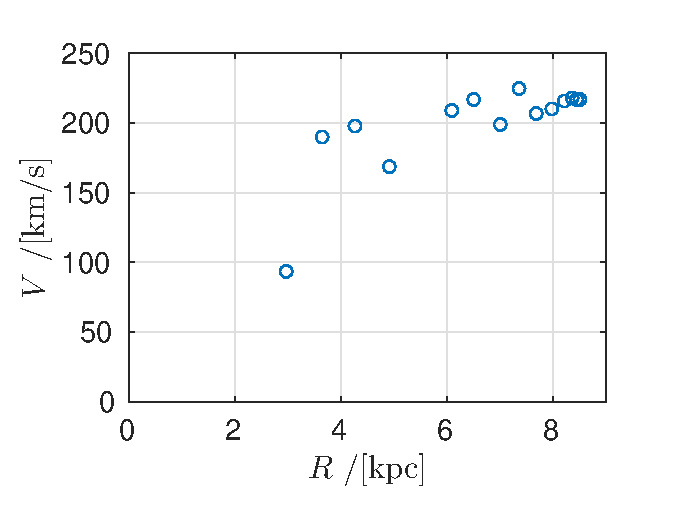
\includegraphics[width=1\linewidth]{rotation_curve.eps}
\caption{Velocity curve for HI clouds in the Milky Way, as observed
  between $20^\circ{-}85^\circ$ Galactic longitude with $5^\circ$
  increments. These velocities are calculated using the circular orbit
  assumption, as well as assuming that the cloud with the highest
  radial velocity is moving tangent to the line of sight.}
\label{fig:rot}
\end{figure}

\begin{figure}\centering
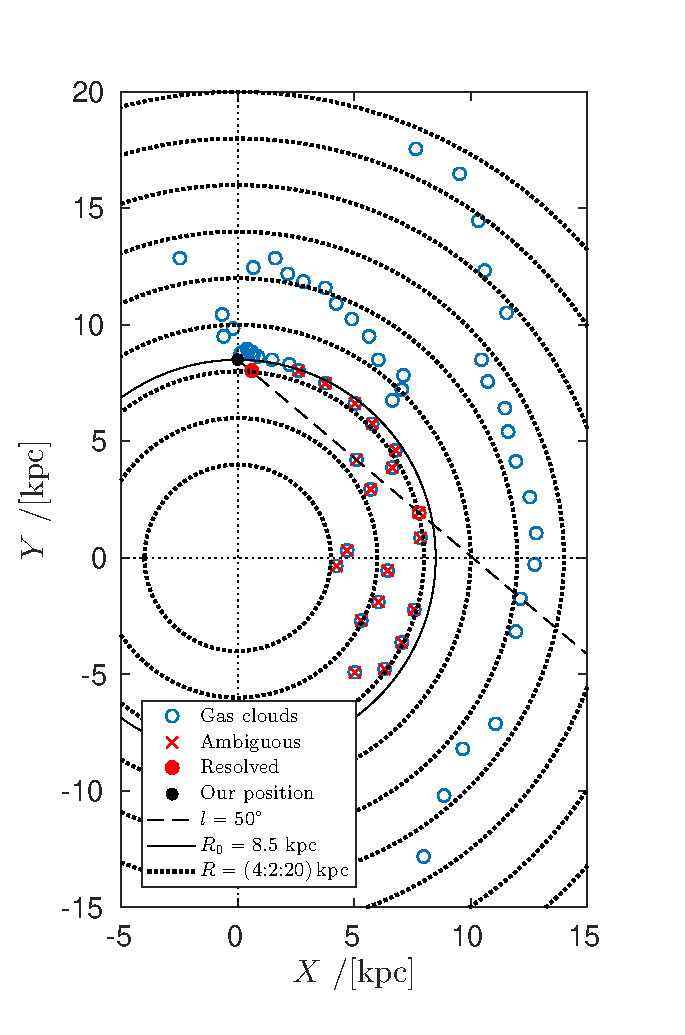
\includegraphics[width=1\linewidth]{gas_clouds.eps}
\caption{Position of HI clouds in the Milky Way. The positions are
  calculated using the assumptions that all clouds have circular
  orbits and that their orbital velocities are
  $V_0=\unit[220]{km/s}$. For some of the clouds there are two
  possible solutions to their position (red crosses). This ambiguity
  problem have been resolved for one cloud on $l=50^\circ$ (red ring,
  correct position filled in). }
\label{fig:clouds}
\end{figure}

\begin{figure}\centering
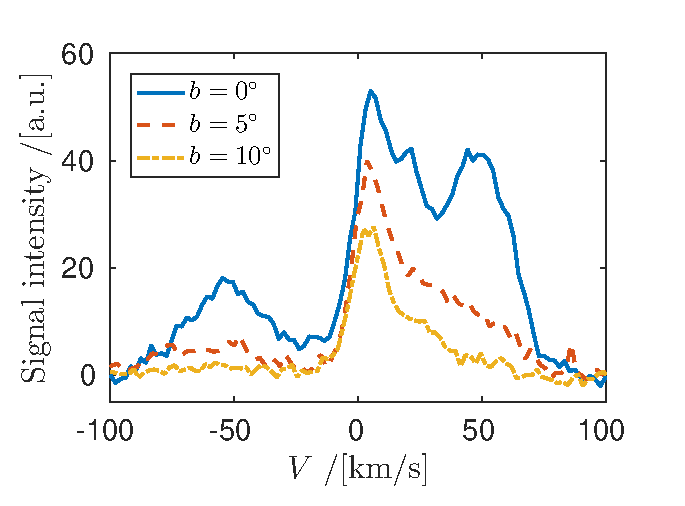
\includegraphics[width=1\linewidth]{ambiguity.eps}
\caption{Velocity spectra to resolve the ambiguity problem for
  $l=50^\circ$. By observing that that the peak near $V=0$ remains for
  different Galactic latitudes, $b$, we can conclude that this gas
  cloud has to be much closer to us than the two others which can be
  seen at $b=0^\circ$. }
\label{fig:ambiguity}
\end{figure}



\section{Conclusions}











%%%%%%%%%%%%%%%%%%%%%%%%%% The bibliography %%%%%%%%%%%%%%%%%%%%%%%%%%
%\newpage
%% This bibliography uses BibTeX
%\bibliographystyle{ieeetr}
%\bibliography{references}%requires a file named 'references.bib'
%% Citations are as usual: \cite{example_article}

%%%%%%%%%%%%%%%%%%%%%%%%%%%%% Appendices %%%%%%%%%%%%%%%%%%%%%%%%%%%%%

%%%%%%%%%%%%%%%%%%%%%%%%%%%%%%%%%%%%%%%%%%%%%%%%%%%%%%%%%%%%%%%%%%%%%%
\end{document}%% ^ ^ ^ ^ ^ ^ ^ ^ ^ ^ ^ ^ ^ ^ ^ ^ ^ ^ ^ ^ ^ ^ ^ ^ ^ ^ ^
%%%%%%%%%%%%%%%%%%%%%%%%%%%%%%%%%%%%%%%%%%%%%%%%%%%%%%%%%%%%%%%%%%%%%%


%%% Local Variables:
%%% mode: latex
%%% TeX-master: t
%%% End:

%  LocalWords:  hyperfine Onsala
